\label{cha:grundlagen}
\chapter{Grundlagen}
Distributed Ledger Technology (DLT) ist ein allgemeiner Begriff für verteilte replizierte Datenbanksysteme, bei denen mehrere Netzwerkknoten ohne zentrale Instanz mittels eines Konsensverfahrens eine gemeinsame konsistente Sicht gespeicherter Transaktionsdaten erstellen \cite{ferdous2020}. Blockchain und Hashgraph, die im Kern diese Arbeit stehen, sind zwei unterschiedliche Datenstrukturen und Konsensmechanismen, mit denen dieses Prinzip umgesetzt wird. Dieses Kapitel führt die konzeptionellen Grundlagen ein, die für das Verständnis der eigentlichen Arbeit benötigt sind. Zuerst werden die Blockchain-Technologie und das darauf aufbauende Hyperledger-Indy/Aries-Ökosystem vorgestellt (Abschnitt~\ref{sec:grundlagen-blockchain}), gefolgt von den Grundlagen des Hashgraph-Konsens und des Hedera Consensus Services (Abschnitt~\ref{sec:grundlagen-hashgraph}). Abschließend werden die Konzepte der Self-Sovereign Identity, der Decentralized Identifiers sowie das Credential-Format AnonCreds beschrieben (Abschnitt~\ref{sec:grundlagen-ssi}).

\section{Blockchain}
\label{sec:grundlagen-blockchain}
In diesem Abschnitt werden zuerst die Grundprinzipien der Blockchain-Technologie eingeführt und anschließend wird mit Hyperledger Indy und Aries das konkrete Blockchain-Ökosystem vorgestellt, auf dem die in dieser Arbeit betrachtete Referenzarchitektur (Abschnitt~\ref{sec:sota_referenzarchitektur}) aufgebaut ist.

\subsection{Grundprinzipien der Blockchain}
Die Blockchain speichert Transaktionen in Blöcken, die kryptographisch miteinander verbunden sind: Jeder Block enthält den Hashwert des vorherigen Blocks, wodurch eine lineare, manipulationsresistente Kette entsteht - nachträgliche Änderungen eines Blocks machen alle nachfolgenden Hashreferenzen ungültig (Abbildung~\ref{fig:blockchain-struktur}). Werden Daten direkt in dieser Kette gespeichert, spricht man von einer On-Chain-Speicherung; werden umfangreiche Daten dagegen außerhalb des Ledgers gehalten und nur ein Verweis oder Hashwert auf dem Ledger verankert, spricht man von einer Off-Chain-Speicherung - ein Muster, das z.B. bei umfangreichen Gesundheitsdaten aus Datenschutz- und Skalierbarkeitsgründen verbreitet ist. \cite{ferdous2020}

\begin{figure}[H]
    \centering
    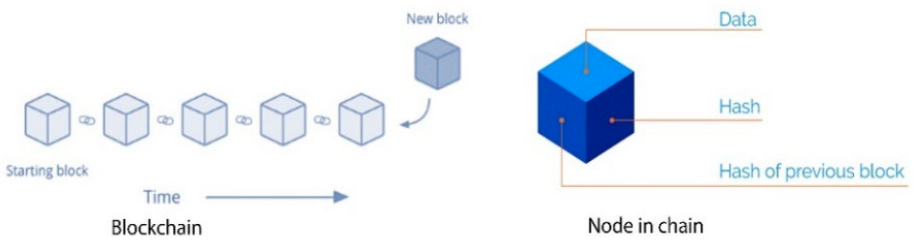
\includegraphics[width=0.5\textwidth]{Figures/hashgraph_vs_blockchain}
    \caption{Blockstruktur einer Blockchain (links) und Aufbau eines einzelnen Blocks (rechts) \cite{alahmad2022}.}    
    \label{fig:blockchain-struktur}
\end{figure}

Um neue Blöcke in dieser Kette zu bestätigen, brauchen die Netzwerkknoten ein Konsensverfahren. Man unterscheidet dabei permissionless Blockchains, an denen beliebige anonyme Teilnehmer ohne Zugangsbeschränkung mitwirken können, von permissioned Blockchains, bei denen eine feste Menge bekannter autorisierter Knoten das Netzwerk bildet. Da bei permissionless Systemen die Teilnehmerzahl unbegrenzt und die Identität der Knoten unbekannt ist, werden dort meistens probabilistische Verfahren wie Proof-of-Work oder Proof-of-Stake eingesetzt, die den Einfluss eines Angreifers künstlich verteuern (Sybil-Resistenz), anstelle einer direkten Abstimmung zwischen bekannten Knoten. In permissioned Blockchains, die in der eigentlichen Arbeit relevant sind, nimmt stattdessen eine feste Menge bekannter autorisierter Knoten über mehrere Kommunikationsrunden eine direkte Abstimmung vor. Abhängig davon, welches Fehlermodell dabei grundlegend ist, unterscheidet man Crash-Fault-Tolerance-Verfahren (CFT), die ausschließlich den Ausfall von Knoten berücksichtigen, von Byzantine-Fault-Tolerance-Verfahren (BFT), die zusätzlich gegen böswillig agierende Knoten robust sind. Klassische BFT-Verfahren wie das Practical Byzantine Fault Tolerance (PBFT) erreichen Konsens, indem die Knoten in mehreren Kommunikationsrunden Nachrichten austauschen und ein Wert erst dann als bestätigt gilt, wenn ihm mehr als zwei Drittel der Knoten zustimmen; solange weniger als ein Drittel der Knoten böswillig ist, bleibt der Konsens dadurch korrekt. \cite{ferdous2020}

\subsection{Hyperledger Indy und Aries im Überblick}
Hyperledger Indy ist eine dezentrale permissioned Blockchain, die ursprünglich vom Unternehmen Evernym speziell für den Aufbau von Identitätssystemen entwickelt und später als Open-Source-Projekt der Hyperledger-Initiative (Linux Foundation) übergeben wurde \cite{sovrin2018}. Das grundlegende Ordnungsprotokoll Indy-Plenum implementiert ein BFT-Verfahren namens RBFT (Redundant Byzantine Fault Tolerance), bei dem eine Gruppe autorisierter Validatorknoten Transaktionen über ein Mehrphasen-Commit-Protokoll ordnet \cite{ferdous2020}. Indy unterscheidet mehrere Ledger-Typen, unter denen der Domain-Ledger für identitätsbezogene Transaktionen eine Schlüsselrolle spielt. Die wichtigsten Transaktionstypen sind NYM (Registrierung öffentlicher DIDs und deren Rollen), SCHEMA (Definition von Attributsätzen für Verifiable Credentials) und CRED\_DEF (Verweis auf ein Schema sowie Aussteller- und Widerrufsinformationen). Die Teilnahme am Netzwerk basiert auf Rollen: Stewards nehmen neue Akteure ins Netzwerk auf, Trust Anchors bzw. Endorser dürfen Schreiboperationen auf dem Domain Ledger durchführen \cite{torongo2023}.

Hyperledger Aries ist ein Agentenframework, das die Kommunikationsschicht zwischen den Identitätsinhabern bereitstellt und dabei Indy als zugrundeliegende Ledger-Technologie nutzt. Es ermöglicht die Ausstellung, Präsentation und den Widerruf von Verifiable Credentials auf Protokollebene, während Indy als vertrauenswürdiger Verankerungspunkt (Trust Anchor) für öffentliche Identitätsinformationen dient. Jeder Teilnehmer wird durch einen Aries-Agenten vertreten, der über eine eigene Wallet - einen sicheren lokalen Speicher für private Schlüssel, DIDs und Credentials - verfügt und mit anderen Agenten über das Protokoll DIDComm verschlüsselte Peer-to-Peer-Nachrichten austauscht. \cite{mazzocca2025}

\section{Hashgraph}
\label{sec:grundlagen-hashgraph}
Dieser Abschnitt führt ein alternatives Konsensverfahren zur Blockchain mit Hashgraph ein und stellt anschließend Hedera als öffentliche Plattform vor, die diesen Konsens implementiert und den zentralen Baustein für den in dieser Arbeit vorgeschlagenen Austausch der Ledger-Schicht mit dem Hedera Consensus Service bereitstellt.

\subsection{Grundprinzipien des Hashgraph-Konsens}
Hashgraph ist ein von Baird \cite{baird2016} entwickelte Datenstruktur, die statt einer linearen Blockkette einen gerichteten azyklischen Graphen (Directed Acyclic Graph, DAG) verwendet - eine Graphenstruktur, deren Kanten jeweils eine Richtung besitzen und die keine Zyklen enthält, sodass man einem Kantenpfad nie zu seinem Ausgangsknoten zurückfolgen kann. Der Hashgraph besteht aus sogenannten Events als Knoten dieses Graphen. Jedes Event enthält null oder mehr Transaktionen, einen Zeitstempel sowie zwei Hash-Referenzen: einen auf das vorherige eigene Event (Self-Parent) und einen auf das letzte von einem anderen Knoten empfangene Event (Other-Parent) \cite{akhtar2019}. Die Verbreitung neuer Events erfolgt über das Gossip-Protokoll, bei dem jeder Knoten periodisch mit einem zufällig gewählten anderen Knoten kommuniziert und ihm alle Events mitteilt, die er noch nicht kennt. Da bei jeder solchen Übertragung nicht nur neue Events, sondern auch die Erkenntnisse darüber, welcher Knoten von welchem Event bereits wusste, weitergegeben wird, spricht man von Gossip about Gossip (Abbildung~\ref{fig:hashgraph-gossip}) \cite{baird2016}.

\begin{figure}[H]
    \centering
    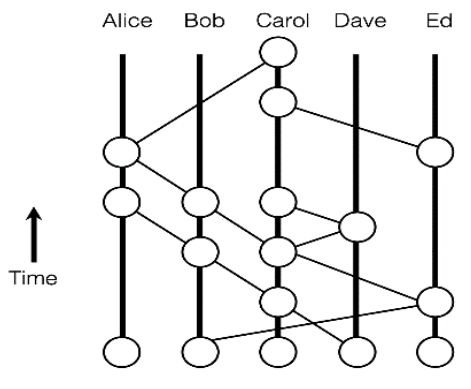
\includegraphics[width=0.6\textwidth]{Figures/hashgraph_gossip_protocol}
    \caption{Gossip-Protokoll im Hashgraph \cite{alahmad2022}.}
    \label{fig:hashgraph-gossip}
\end{figure}

Anhand der so entstehenden Graphenstruktur lässt sich rekonstruieren, welche Events einem Knoten zu welchem Zeitpunkt bereits bekannt waren. Dadurch kann jeder Knoten lokal berechnen, wie die anderen Knoten abstimmen würden, ohne dass tatsächlich Abstimmungsnachrichten ausgetauscht werden müssen - dieses Verfahren wird als Virtual Voting bezeichnet \cite{baird2016, alahmad2022}. Darauf basierend wird eine konsistente Reihenfolge und ein konsistenter Zeitstempel (Median der beobachteten Zeitstempel) für jedes Event berechnet. Baird beweist formal, dass dieses Verfahren asynchron byzantinisch fehlertolerant (aBFT) ist: Solange mehr als zwei Drittel der Knoten korrekt arbeiten, wird auch unter beliebigen Netzwerkverzögerungen ein korrekter, fairer Konsens erreicht \cite{baird2016}.

\subsection{Hedera als Plattform und Hedera Consensus Service}
Hedera ist ein 2018 von Leemon Baird und Mance Harmon \cite{bairdharmon2019} gegründetes öffentliches Netzwerk, das den Hashgraph-Konsens als Grundlage verwendet. Die Konsensknoten werden dabei von den Mitgliedsorganisationen des Hedera Governing Council betrieben; Nutzer greifen stets auf dieses eine öffentliche Netzwerk zu, anstatt eine eigene lokale Instanz zu betreiben \cite{bairdharmon2019}. Auf der Konsensebene setzt eine Services-Ebene auf, die unter anderem den Hedera Consensus Service (HCS) bereitstellt \cite{bairdgross2019}. HCS unterscheidet sich grundlegend von klassischen Ledgern, die den Zustand direkt speichern: Es handelt sich um einen reinen Ordnungs- und Zeitstempeldienst. Anwendungen erstellen dafür einen sogenannten Topic (identifiziert durch eine Topic-ID) und senden Nachrichten an diesen Topic. Das Hedera-Netzwerk ordnet diese Nachrichten mittels Hashgraph-Konsens in eine faire manipulationsresistente Reihenfolge an und weist jeder Nachricht einen Konsens-Zeitstempel zu, speichert den Inhalt der Nachrichten selbst jedoch nicht dauerhaft im Sinne eines Anwendungszustands.

Mirror Nodes werden eingesetzt, um aus dem geordneten Nachrichtenstrom eines Topics einen Anwendungszustand wiederherzustellen; das sind rein lesende Knoten, die den Nachrichtenstrom vom Hedera-Netzwerk empfangen, jedoch nicht am Konsens teilnehmen. Eine Anwendung, die aus einem oder mehreren Topics und einer Menge zugehöriger Mirror Nodes bzw. Client-Anwendungen besteht, wird als Appnet bezeichnet. Das Appnet-Muster erlaubt es, die Ausführung und Zustandsspeicherung einer Anwendung vollständig off-chain zu belassen, während lediglich die Reihenfolge und Integrität der zugrunde liegenden Events durch das öffentliche Hedera-Netzwerk geschützt wird. \cite{bairdgross2019}

\section{Self-Sovereign Identity und Decentralized Identifiers}
\label{sec:grundlagen-ssi}
Dieser Abschnitt führt das Paradigma der Self-Sovereign Identity ein und stellt die zugrundeliegenden technischen Bausteine vor: Decentralized Identifiers, Verifiable Credentials, deren Ausprägung als AnonCreds sowie das DIDComm-Kommunikationsprotokoll.

\subsection{Das SSI-Paradigma}
Self-Sovereign Identity (SSI) ist ein Identitätsmanagement-Paradigma, bei dem Nutzer die vollständige Kontrolle über ihre eigenen Identitätsdaten behalten, anstatt sie bei zentralen Identitätsanbietern zu speichern \cite{mazzocca2025}. Historisch kann SSI als dritte Entwicklungsstufe des digitalen Identitätsmanagements einordnet werden: Auf zentralisierte Modelle, bei denen jeder Dienst eigene Konten verwaltet, folgten föderierte Modelle mit übergreifenden Identitätsanbietern, und schließlich SSI, das ohne eine zentrale verwaltende Instanz funktioniert \cite{mazzocca2025}. Die Sovrin Foundation hat hierzu wichtige Ziele formuliert, wie Sicherheit (Schutz der Identitätsdaten vor unerwünschter Offenlegung), Kontrollierbarkeit (der Identitätsinhaber bestimmt, wer auf welche Daten zugreift) und Portabilität (Identitäten sind nicht an einen Anbieter gebunden) \cite{sovrin2018}.

Die Interaktion in SSI-Systemen erfolgt im Rahmen der sogenannten Trust Triangle aus drei Rollen: Ein Issuer stellt einem Holder eine digital signierte Bescheinigung aus, die der Holder in seiner eigenen Wallet hält und bei Bedarf einem Verifier präsentiert. Der Verifier prüft die Bescheinigung kryptographisch gegen öffentlich verfügbare Informationen des Issuers, ohne diesen direkt kontaktieren zu müssen \cite{mazzocca2025}. Eine verteilte, manipulationsresistente Registry - typischerweise ein Distributed Ledger - dient dabei als gemeinsamer Vertrauensanker, auf dem die öffentlichen Schlüssel und Definitionen der Issuer gespeichert sind \cite{sovrin2018}.

\subsection{Decentralized Identifiers und DID-Documents}
Decentralized Identifiers (DIDs) sind global eindeutige vom W3C standardisierte Identifikatoren, die ohne zentrale Registrierungsstelle generiert und aufgelöst werden können. Eine DID verweist auf ein DID-Document: eine JSON-Datenstruktur, die die öffentlichen Schlüssel des Identitätsinhabers sowie Service-Endpunkte für die Kommunikation mit ihm enthält. Die Auflösung einer DID zu ihrem DID-Document erfolgt über eine sogenannte DID-Methode, die definiert, in welcher Registry (z.B. einem bestimmten Distributed Ledger) das Dokument gespeichert ist und wie es erzeugt, aktualisiert und deaktiviert wird. Zusätzlich zu den öffentlich auf einem Ledger verankerten DIDs existieren auch Peer-DIDs, die nur zwischen zwei Kommunikationspartnern ausgetauscht und nicht auf einem Ledger registriert werden - ein Ansatz, der die Registry entlastet und die Privatsphäre erhöht, da paarweise Beziehungen nicht öffentlich zugänglich sind. \cite{mazzocca2025}

\subsection{Verifiable Credentials}
Verifiable Credentials (VCs) sind ein ebenfalls vom W3C standardisierte Datenformat für den Austausch von Identitätsattributen im SSI-Modell \cite{mazzocca2025}. Ein VC enthält eine Menge von Aussagen (Claims) über ein Subjekt, die vom Issuer digital signiert werden. Der Lebenszyklus eines VC umfasst drei Phasen: die Ausstellung (Issuance) durch den Issuer an den Holder, die Präsentation (Presentation) durch den Holder gegenüber einem Verifier sowie gegebenenfalls den Widerruf (Revocation) durch den Issuer. Bei der Präsentation sind keine vollständige Credential erforderlich: Verfahren wie Selective Disclosure und Zero-Knowledge-Proof erlauben es dem Holder, nur einzelne Attribute oder abgeleitete Aussagen nachzuweisen \cite{mazzocca2025}. Für den Widerruf werden meistens kryptographische Akkumulatoren verwendet, die es einem Verifier ermöglichen, die Gültigkeit eines Credentials gegen eine öffentliche Widerrufsregistratur zu prüfen, ohne dass der Issuer einzelne Widerrufe personenbezogen offenlegen muss \cite{torongo2023}..

\subsection{AnonCreds als Credential-Format}
\label{subsec:grundlagen-anoncreds}
Das W3C-Datenmodell für Verifiable Credentials legt nur fest, welche Bestandteile ein Credential enthält, nicht jedoch, mit welchem kryptographischen Verfahren es signiert und geprüft wird. Anonymous Credentials (AnonCreds) sind eine konkrete Umsetzung dieses Datenmodells, die ursprünglich im Rahmen von Hyperledger Indy entstanden ist und inzwischen als eigenständige Spezifikation geführt wird \cite{anoncredsspec}. AnonCreds verwendet CL-Signaturen (Camenisch-Lysyanskaya), die es dem Holder erlauben, aus einem ausgestellten Credential eine Präsentation abzuleiten, in der nur ausgewählte Attribute offengelegt werden (Selective Disclosure) und in der Prädikate über Attribute als Zero-Knowledge-Proof nachgewiesen werden können, ohne den Attributwert selbst öffentlich zu machen \cite{anoncredsspec}. Außerdem verbindet ein sogenanntes Link Secret das Credential mit Holder, ohne dass dieser Wert dem Issuer bekannt wird, wodurch Präsentationen desselben Credentials nicht miteinander korreliert werden können \cite{anoncredsspec}.

Für die eigentliche Arbeit ist es wichtig, welche Objekte AnonCreds außerhalb der Wallet des Holders behalten muss. Die Spezifikation definiert vier Objekttypen, die öffentlich auflösbar sein müssen: Schema (Menge der Attributnamen), Credential Definition (die vom Issuer verwendeten öffentlichen Schlüssel mit Verweis auf ein Schema), Revocation Registry Definition sowie die ständig aktualisierten Revocation Status Lists, die den Zustand des kryptographischen Akkumulators führen \cite{anoncredsspec}. Diese Objekte bilden genau die Inhalte, die in der Referenzarchitektur auf der Ledger-Schicht abgelegt werden.

\subsection{DIDComm als Kommunikationsprotokoll}
DIDComm ist ein Protokoll für eine verschlüsselte, transportunabhängige Peer-to-Peer-Kommunikation zwischen SSI-Agenten \cite{mazzocca2025}. Die Verschlüsselung und Authentifizierung der Nachrichten basiert direkt auf den in den DID-Documenten gespeicherten Schlüsseln der Kommunikationspartner, wodurch keine zusätzliche Public-Key-Infrastruktur benötigt wird. Auf DIDComm bauen höhere Protokolle für die Ausstellung und Präsentation von Verifiable Credentials auf. Da DIDComm ausschließlich DIDs und deren Schlüsselmaterial verwendet, ist es unabhängig von der konkreten Registry, in der öffentliche DIDs gespeichert sind  - eine Eigenschaft, die für den in dieser Arbeit betrachteten Austausch der Ledger-Schicht eine zentrale Rolle spielt.

